After having modelled the source and its materials, the MCNP simulation runs the described source placed 2.65 \unit{\centi\meter} away from the outermost part of the ionization chamber in its transversal direction and pointing to the chamber. Finally, the geometry of the source was replicated using translation cards of MCNP in its mirror position to match the experimental configuration. The view in the \emph{XY} plane of the arrangement set to run at the desired number of particles is: 

\begin{figure}[!h]
    \centering
    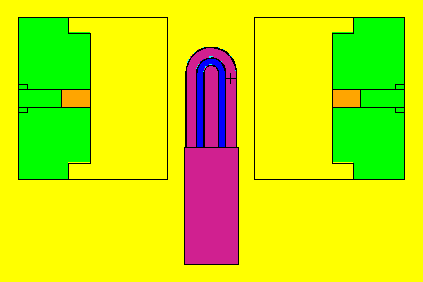
\includegraphics[scale = 0.9]{Master Thesis Manuel Galdon/figures/sr-90_full_setup.PNG}
    \caption{Geometrical arrangement of the simulated \ce{^{90}{}Sr} source and the PTW TM33054 magnesium chamber.}
    \label{fig:Sr90_full_setup}
\end{figure}

\clearpage
The closest line of the source to the chamber is not a wall and must not be understood as an edge with which the particles interact once they are emitted. Planes are meant to define the cells and are not made of any material themselves. The line is just an MCNP plane that needs to be set up to define the cell and fill it with air. 

%Of course, there is a slight deviation between the geometry of the simulated source and the sketch depicted in Figure \ref{fig:PTW sketch and simulation}. These are small differences that only affect the edges of the brass structure. However, the cylindrical geometry of the brass and strontium cells has been preserved as much as possible to adhere to the actual device features. 
Both sources and the chamber are placed in a wooden structure that holds all three devices in the presented position and given the dimensions of the setup, the presence of the frame will not produce a measurable significant effect in the dose deposited in the argon gas inside the chamber. 

For security reasons and due to the regulations of \emph{FRM II} regarding the access to the facilities, it is unfortunately not possible to include in the present work a photo of the actual set of frame, sources and chamber to evidence its differences with our simulation. 

To visualize the particle flux in the MCNP geometry, the simulation needs to be run using the \emph{FMESH} card. It sets a grid around the entire setup. The result of the test is:

\begin{figure}[!h]
    \centering
    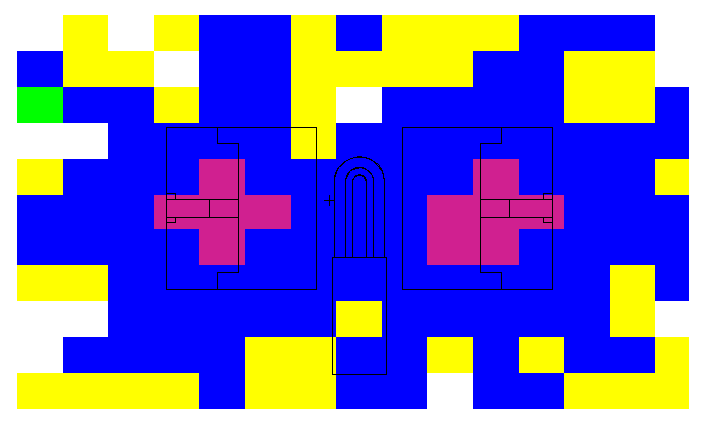
\includegraphics[scale = 0.7]{Master Thesis Manuel Galdon/figures/void_setup.png}
    \caption{Particle flux in empty geometry.}
    \label{fig:Particle flux in a void geometry}
\end{figure}

The interpretation of Figure \ref{fig:Particle flux in a void geometry} relies on understanding the color scheme employed by MCNP. The color purple is assigned to the region with the highest particle concentration, while blue, yellow, and green represent progressively lower incidences of particles. In Figure \ref{fig:Particle flux in a void geometry} it is evidenced that any intensity of the flux of particles that stems from the cells where the source is set up lies around that cell and propagates towards the position of the chamber. Hence, all cells are geometrically correct and the simulation is ready to run.